% !TeX document-id = {55487e37-df6e-4d5b-af2f-b0275db5df41}
%%
%% This is file `sample-manuscript.tex',
%% generated with the docstrip utility.
%%
%% The original source files were:
%%
%% samples.dtx  (with options: `manuscript')
%% 
%% IMPORTANT NOTICE:
%% 
%% For the copyright see the source file.
%% 
%% Any modified versions of this file must be renamed
%% with new filenames distinct from sample-manuscript.tex.
%% 
%% For distribution of the original source see the terms
%% for copying and modification in the file samples.dtx.
%% 
%% This generated file may be distributed as long as the
%% original source files, as listed above, are part of the
%% same distribution. (The sources need not necessarily be
%% in the same archive or directory.)
%%
%% The first command in your LaTeX source must be the \documentclass command.
%%%% Small single column format, used for CIE, CSUR, DTRAP, JACM, JDIQ, JEA, JERIC, JETC, PACMCGIT, TAAS, TACCESS, TACO, TALG, TALLIP (formerly TALIP), TCPS, TDSCI, TEAC, TECS, TELO, THRI, TIIS, TIOT, TISSEC, TIST, TKDD, TMIS, TOCE, TOCHI, TOCL, TOCS, TOCT, TODAES, TODS, TOIS, TOIT, TOMACS, TOMM (formerly TOMCCAP), TOMPECS, TOMS, TOPC, TOPLAS, TOPS, TOS, TOSEM, TOSN, TQC, TRETS, TSAS, TSC, TSLP, TWEB.
% \documentclass[acmsmall]{acmart}

%%%% Large single column format, used for IMWUT, JOCCH, PACMPL, POMACS, TAP, PACMHCI
\documentclass[acmlarge,screen]{acmart}
% !TeX TXS-program:compile = txs:///pdflatex/[--shell-escape]

%%%% Large double column format, used for TOG
%\documentclass[acmtog, authorversion]{acmart}

%%%% Generic manuscript mode


%%
%% \BibTeX command to typeset BibTeX logo in the docs
\AtBeginDocument{%
  \providecommand\BibTeX{{%
    \normalfont B\kern-0.5em{\scshape i\kern-0.25em b}\kern-0.8em\TeX}}}

\usepackage{listings}
\usepackage{minted} 
\usepackage{subcaption}
\usepackage{float}
\usepackage{wrapfig}
\restylefloat{figure}
\usemintedstyle{friendly}
\graphicspath{ {../images/} }



%%
%% The majority of ACM publications use numbered citations and
%% references.  The command \citestyle{authoryear} switches to the
%% "author year" style.
%%
%% If you are preparing content for an event
%% sponsored by ACM SIGGRAPH, you must use the "author year" style of
%% citations and references.
%% Uncommenting
%% the next command will enable that style.
%%\citestyle{acmauthoryear}

%%
%% end of the preamble, start of the body of the document source.
\begin{document}

%%
%% The "title" command has an optional parameter,
%% allowing the author to define a "short title" to be used in page headers.
\title{UVU MCS Graduate Paper}

%%
%% The "author" command and its associated commands are used to define
%% the authors and their affiliations.
%% Of note is the shared affiliation of the first two authors, and the
%% "authornote" and "authornotemark" commands
%% used to denote shared contribution to the research.

\author{Benjamin Stoneking}
\affiliation{%
 \institution{Candidate}
}
\email{benjamin.stoneking@protonmail.com}

\author{Frank Jones}
\affiliation{%
 \institution{Advisor}
}
\email{frankj@uvu.edu} 

%%
%% By default, the full list of authors will be used in the page
%% headers. Often, this list is too long, and will overlap
%% other information printed in the page headers. This command allows
%% the author to define a more concise list
%% of authors' names for this purpose.
\renewcommand{\shortauthors}{Candidate First Last}

%%
%% The abstract is a short summary of the work to be presented in the
%% article.
\begin{abstract}
	The project explores the implementation of an embedded real-time digital audio synthesizer. Emphasis is placed on leveraging the inherent strengths of the hardware (timers, hardware interrupts, etc) to produce a reliable musical instrument. The project is a focused exercise in implementing a digital audio processing pipeline with software implementations of common components such as oscillators, pitch control, signal gain attenuation, and filtering. It illustrates the process of implementing a capable, complex and extendable embedded system on a platform with limited processing power. The final product is a fundamental subtractive synthesizer: It responds to input from generic MIDI devices to produce an audio signal. It applies volume dynamics and timbre control to the signal using envelopes and filters. The device has a hardware interface consisting of knobs, encoders, and a screen allowing direct, real-time manipulation of the processing. A PC application can control the system remotely. The system is robust and extensible. Numerous features can be added. The project code base was written with to be efficient in its size and speed. The project firmware source is about 2,000 lines with with PC application and test code bringing it up to 2,500.
\end{abstract}

%%
%% Keywords. The author(s) should pick words that accurately describe
%% the work being presented. Separate the keywords with commas.
\keywords{digital, audio, synthesis, embedded, microcontroller, real-time, midi, hardware, oscillator, filter, envelope, DSP, prototype, discrete-time, continuous-time, analog}

%%
%% This command processes the author and affiliation and title
%% information and builds the first part of the formatted document.
\maketitle

\section{Introduction}
\subsection{Purpose}
	The acquisition of musical gear is a common obsession that plagues millions of musicians around the world. The cost of gear for performance or music production presents a major financial struggle to musicians already working with a tight budget. A common thought occurs to musicians: "What if I just make my own X? Maybe I can save some money." This discussion occurs frequently within online and offline discourse. Often, musicians who have experience making their own digital or analog instruments give the same answer: "Yes. You can just make your own X. But no. You won't save any money. You will end up spending more and you should just save up some cash to just buy your gear." I've walked this path myself and found this conclusion to be true but with a small caveat: You can in fact save money by making your audio production tool as a \textbf{digital system}. You can write as much software as you want. You can refactor and rebuild you software tool over and over, and never spend a dime. When physical electronic components are removed from the equation, you can make all your music production gear for free. This caveat has a caveat of its own: This takes substantial time. Time is money. Therefore, every hour spent in implementing your system is implicitly adding to the hypothetical price tag of your system.
	
	Of course, implementing your own digital audio processing tools can be seen as reinventing the wheel. This project can be characterized as \textit{yet another} software synthesizer. The purpose of this project is not to create a product that is competitive with the mainstream market, but to discover the process and patterns of building an audio synthesis system on an embedded platform. My education has had me walk through the process of making \textit{yet another} database management system, and \textit{yet another} virtual machine. Unsurprisingly, my database hasn't replaced MySQL and my virtual machine has not replaced the Java Virtual Machine. Reinventing the proverbial wheel does not make the effort fruitless. Valuable wisdom and knowledge of how complex systems work is gained on the journey to replicate existing solutions. I applied this same principle to my master's project: Make \textit{yet another} digital synthesizer on an embedded microcontroller. \textbf{The endgame of this project is the journey itself}:
	\begin{itemize}
		\item Learn how to implement a complex real-time embedded system
		\item Develop a modular digital audio pipeline
		\item Build a hardware interface to control the system
		\item Discover what invaluable knowledge can be extracted from the experience
	\end{itemize}
	The aim of this project was to accomplish the task of creating this device, document the architecture, process and the lessons learned. What is a valid working architecture to making such a system? Where does one begin? What kind of failure and setbacks should be expected? Can it be done within a reasonable amount of time without substantial reliance on previously existing frameworks and libraries? What sort of mathematical and technical knowledge is required?

\subsection{Project Criteria}
	\subsubsection{Minimum Requirements}
	\label{requirements}
	This implementation of a subtractive synthesizer must meet the following minimum requirements (see Concepts for definitions):
	\begin{enumerate}
		\item Produce audio at a minimum quality of 44.1khz and 16 bit-depth (Industry standard quality)
		\item Compatible with any generic MIDI keyboard.
		\item \textbf{Oscillator} module must generate the most common wave forms: Sin, sawtooth, square, triangle and white noise
		\item Support polyphony, with capability to play up to eight discrete notes at a time.
		\item Support mixing of multiple oscillators to generate hybrid waveforms.
		\item Support \textbf{envelope} signal generation for dynamic modulation of other signals.
		\item Implement a\textbf{Filter} module that supports lowpass, highpass and bandpass filtering, able to adjust frequency cutoff and resonance in real-time.
		\item Implement \textbf{low-frequency oscillator (LFO)} module configurable to modulate the signals of other modules within the system.
		\item Provide a memory bank where users can save their "patches" to use later.
		\item Provide interaction between the user and the system via a \textbf{hardware interface}. User inputs include a MIDI jack for keyboard input and knobs for navigating a menu and changing parameters. Outputs include a 1/8" audio output jack for playback with headphones and speakers and a menu screen for communicating the system state to the user. Knobs adapt to the context of the menu to appropriately adjust parameters.
	\end{enumerate}
	
	\subsubsection{Constraints}
	In order to maximize the learning potential of this project and focus on the process rather than the final destination, I set a few restrictions:
	\begin{enumerate}
		\item Language: Implement the firmware in a low-level programming language such as C/C++. Complex, non-static data structures should be avoided to keep the system efficient, transparent and stable.
		\item Libraries: Utilize only the standard C/C++ libraries with the exception of a Hardware Abstraction Layer to minimize hardware peripheral set up time. 
		\item References: Put forth every effort to learn the mathematical concepts of DSP and implement them without referencing existing solutions.
	\end{enumerate}
	
\subsection{Results}
	\subsubsection{What did I learn?}
	
	\paragraph{Choose your device platform carefully} I chose the audio development board Daisy by Electro-Smith. It is marketed as an attractive option for musicians to implement their dream systems because of its high resolution digital to analog (DAC) converter and painless hardware peripheral abstractions. It turned out to not be as mature and stable as I hoped and had many issues with drivers, pin connections and lacking support for certain interrupt service routines. Initially, it was difficult to see that Daisy may not have been the best option for implementing a system scoped beyond a hobbyist project. The platform was designed for musicians to implement simpler systems with highly abstracted development libraries and programming languages/frameworks like MaxMSP, Puredata and Arduino. More attention and care was put into supporting these tools and making them work well while some lower level capabilities were sidelined.
	
	\paragraph{Prototype hardware incrementally} After spending several months setting up my hardware peripherals on a breadboard and implementing core functionality, I felt the need to migrate the system off a breadboard to a more permanent and stable fixture. It was at this point I learned the cost of trying to do too much at once. I tried to design a soldered circuit board able to be embedded in an enclosure that was yet to be designed. My thought was that it may take several revisions of the enclosure before I knew where all my knobs, encoders, inputs, outputs and screen needed to be for ease of use and optimal functionality. I built up flying wire harnesses for all peripherals so that they could be moved around to test out different enclosure layouts. The result was an absolute mess of wires that were susceptible to interference. My first step in taking the system off the breadboard should have been simply solder my components into logical sections on perf board and make the system work as it did on the breadboard. It would not have been an optimal design and I would have to do another revision to get the system installed in an enclosure. But I would have saved so much time soldering and troubleshooting a sloppy design that ultimately failed. More time could have been allocated to adding additional capabilities to the software.
	
	\paragraph{Decouple pure software functions from hardware and test independently} My workflow for the entirety of the project was \textbf{write code, compile, flash, test, repeat}. This involves a lot of waiting. Waiting for the compiler. Waiting for the bootloader. Waiting for the flash process to complete. If I wrote my code more carefully to not be so tightly coupled to the Daisy system, I could have written some pure software test fixture code that runs on my host PC to test my different synth components independently. It would facilitate a much tighter development and testing loop. In addition, the modules would be more portable and easy to integrate into other systems.
	
	\paragraph{Purchase hardware components from trusted sources and verify functionality} I made the mistake of sourcing some components from Amazon. The cheap price and quick delivery was too much of a temptation. I ended up wasting several agonizing days troubleshooting and debugging software all because of one encoder in a bag of ten. The factory happened to solder its PCB in reverse and it was completely defective. I assumed my code was the problem. Only after hooking the offending part up to a multimeter was I able to see the problem. I replaced the part and my system worked without a single change to the software. It resonable good to suspect your implementation may be flawed before blaming hardware. Manufactured parts should be trusted, but also verified.
	
	\subsubsection{Complexity}
	\paragraph{Looking at the code does not always accurately express the effort and time invested to develop a solution}. Writing driver code for the project was a long process. It required reading long data sheets for devices and how they work. Each component requires a surprisingly deep level of knowledge to properly communicate with them. Actually writing the code to communicate in the devices specific protocol can be long process of trial and error. 
	
	\paragraph{Implementing the driver code to communicate with the LCD screen over I2C took a couple weeks} Many hours of time were spent writing low level functions to pack a lot of information into just several bytes of data that perform one function. These functions need to be written to perform an insignificant task like writing a single character to the screen, moving the cursor, erasing the screen or just configure the screen. More functions need to be written using these new driver level functions to do things like write a complete string to a specific line or create a menu scrolling effect. After all this time is spent implementing these necessary functions, the driver code may only be one or two hundred lines long. This experience demonstrates the fact that lines of code is not an accurate model for determining the complexity of a system.
	
	\subsubsection{Design decisions}
	\paragraph{The final architecture of the system as a whole cannot described perfectly with one model} It is a hybrid of several architectures. The system is \textbf{pipeline architecture}. Synth modules are chained together in a mostly linear fashion. Oscillators generate audio sample data. Samples from multiple oscillators are attenuated and combined into a new sample. The aggregated sample is passed through an envelope modulated attenuator. The sample is then passed to a filter. The filtered samples are passed through an audio fx chain where each effect module processes and passes data down to the next. The samples processed by the fx chain are passed through a master volume attenuator and put into the audio DAC's output buffer. The DAC finally converts the digital signal to an analog signal which plays out the physical speakers.
	
	It is an \textbf{event driven architecture}. The audio DAC interrupt drives the audio processing of the synthesizer pipepline. It is responsible for acquiring a sample from the synth and placing it into the DAC's output buffer (note how the DAC functions both as an event driver and as a component in the pipeline). The hardware timer interrupt processes user input. It uses the processed user input to control the various synth components. Because it runs much slower than the DAC, it also drives some synthesizer components like the envelope which generate modulation source signals rather than audio.
	
	It is also a \textbf{modular architecture}. Although modularity is a basic expectation of software design, it plays a much bigger role in synthesis itself. It has been a fundamental principle in synthesis since day one. The first synthesizers were a collection of analog circuit boards completely divorced from one another, and they were only connected by series of physical patch cables that could be endlessly rerouted in different permutations. This core principle is implemented into the software. The data structures are independent modules: oscillators, filters, envelopes and LFOs all able to connect to each other similar to how analog synthesizers are connected by patch cables. This aspect of the system obscures some of the pipeline nature of the software architecture, because the system is just a linear chain of single file units. Some modules are abstract components, aggregating smaller modules to achieve new functionality. Some modules like the envelope do not directly process audio. Instead, they generate signals parallel to the audio pipeline that affect how \textit{other} modules process data. 
	
	The software architecture does not entirely fit a single model, but is a combination of architectures and in some ways blurs the lines that distinguish them.

\section{Related Works}
	\begin{description}
		\item[Designing Sound by Andy Farnell] A practical guide to digital audio synthesis. Describes the common structures of DSP using a visual programming language called PureData. Used as primer for understanding modules implemented in this project.
		\item[Think DSP: Digital Signal Processing in python by Allen Downey] DSP examples written in python. Referenced for generating oscillator functions and understanding concepts of filtering.
		\item[Embedded Systems Architecture by Daniele LaCamera] Comprehensive textbook on embedded systems. Heavily referenced for hardware configuration and firmware design.
		\item[Audio effects: Theory, implementation, and application by Joshua Reiss and Andrew McPherson] References in implementations of audio fx (filters, reverb, delay, phaser etc). Referenced for planned but yet unimplemented audio fx chain.
		\item[Subtractive synthesis: The synthesizer academy by Scott Rise] Blog post on subtractive synthesis. Referenced as industry definition of subtractive synthesis and its applications.
		\item[Learning synthesis: Oscillators by Eldar Tagi] Blog post explaining different types of oscillators, waveforms and their implementations in analog and digital domain. Referenced for study of the history of synthesis, definition of frequency modulation and the functions of oscillators.
		\item[microKorg by Korg] A compact polyphonic analog synthesizer. An industry standard instrument used as a reference when defining the requirements of the project.
		\item[What is a LFO and how to use it by Vanesa Paris] A blog post explaining the mechanics and applications of Low Frequency Oscillators. A reference for the requirements of the unimplemented LFO module.
		\item[Midi for the Arduino - Build a Midi Input Circuit] A blog post explaining how to implement an optocoupler protected midi input circuit to an Arduino. This circuit was implemented in its entirety and adapted to work with the Daisy platform.
		\item[Materials for Linear Algebra: Linear Filters by Joshua Holden] A free Duke University text book referenced extensively for understanding discrete time signal filtering with difference equation.
		\item[Introduction to Digital Filters with Audio Applications by Julius Smith] A free Stanford University textbook on Digital Filters. Referenced heavily for learning about transfer functions, bilinear transform and second order difference equation.
		\item[Introduction to Computer Music by Jeffrey Hass] Indiana University text book covering analog and digital synthesis concepts, filters, envelopes, etc. Very comprehensive and referenced for research on envelopes, filters and oscillators.
		\item[libDaisy by Electro-Smith] Open source hardware abstraction layer library for the Daisy ecosystem. Heavily used in implementation for settings up DAC/Timer interrupts, potentiometer ADCs, digital encoder reading and I2C bus setup.
		\item[Welsh's synthesizer cookbook by Fred Welsh] A "cookbook" for setting up any generic synthesizer to emulate sounds like pianos, violins, banjo, guitar etc. Referenced for researching concepts of subtractive synthesis.
		\item[The MIDI Manual by David Miles Huber] A comprehensive textbook covering the MIDI protocol. Referenced for explanations of how data is packed into MIDI messages.
	\end{description}

\section{Concepts}
	\begin{itemize}
		\item \textbf{Oscillator:} Generally speaking, an oscillator is a function generator. Generates a repeating signal at a specified frequency much like the function generator of an oscilloscope. The starting point of the audio signal chain.
		\item \textbf{Monophonic:} A synth that can play only one pitch at a time.
		\item \textbf{Polyphonic:} A synth that can play two or more discrete notes at a time.
		\item \textbf{Voice:} A structure containing one or more oscillators. One voice can play one pitch at a time. Voices are used to support polyphony.
		\item \textbf{Modulation:} The usage of an analog or digital signal as a function to alter the inputs of another function.
		\item \textbf{Envelope:} A multiphase linear signal generator. Used as a modulation source for other signals.
		\item \textbf{Low Frequency Oscillator (LFO):} An oscillator producing signals below human hearing. Used as a modulation source.
		\item \textbf{Low Pass Filter:} A filter that removes high frequencies from a signal past a certain cutoff point.
		\item \textbf{High Pass Filter:} Like a low pass filter but removing low frequencies.
		\item \textbf{Sample Rate:} Refers to how often a digital signal is being sampled in samples per second.
		\item \textbf{Bit Depth:} How many bits are used to represent a digital sample.
		\item \textbf{Digital to Analog Converter (DAC):} A hardware component used to output a digital signal as an analog voltage signal.
		\item \textbf{MIDI:} Musical Instrument Data Interface. A communications protocol for controlling electronic instruments, computer software, lighting systems etc. Supports hundreds of different kinds of messages. "Note On" and "Note Off" messages are the most common and contain pitch and velocity (how loudly the note is being played).
		
		
	\end{itemize}

\section{Software Architecture and Implementation}

\subsection{A High Level View}
	\paragraph{As mentioned previously, the system is an interrupt driven, highly modular, pipeline architecture} A class called synth is a composition of modules that connect to form an digital audio processing pipeline. Two interrupt service routines function as the main operators of this pipeline: A \textbf{hardware timer} interrupt is responsible for capturing user input to control the synths parameters and the notes it plays. An \textbf{audio} interrupt, triggered by the high resolution DAC is responsible for driving the pipeline to generate digital audio samples and load the samples into the DAC's audio out buffer.
	
	There are five key participants involved in the system:
	\begin{enumerate}
		\item The \textbf{user} operating the system with the keyboard keyboard and hardware peripherals
		\item The \textbf{menu system} communicating the system state to the user
		\item The \textbf{synth} generating audio samples for the DAC
		\item The \textbf{timer interrupt} reading hardware inputs to trigger events
		\item The \textbf{audio interrupt} requesting the next sample to write to the audio output DAC.
	\end{enumerate}

%	\begin{figure}[h]
%		\centering
%		\caption{This sequence is the most common event for the runtime of the system. It represents the idle state when the user is not engaged in the system. The process audio callback is continuously requesting samples from the synth, and the synth is just returning a value of zero. The result is silence for the user. \textit{Note: although the timer appears in active, the interrupt is still occuring with no inputs to detect to trigger events.}}
%		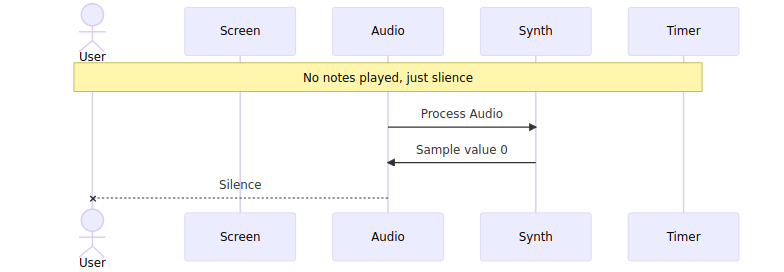
\includegraphics[width=.7\linewidth]{no_note_sequence}
%	\end{figure}

	\begin{figure}[H]
		\centering
		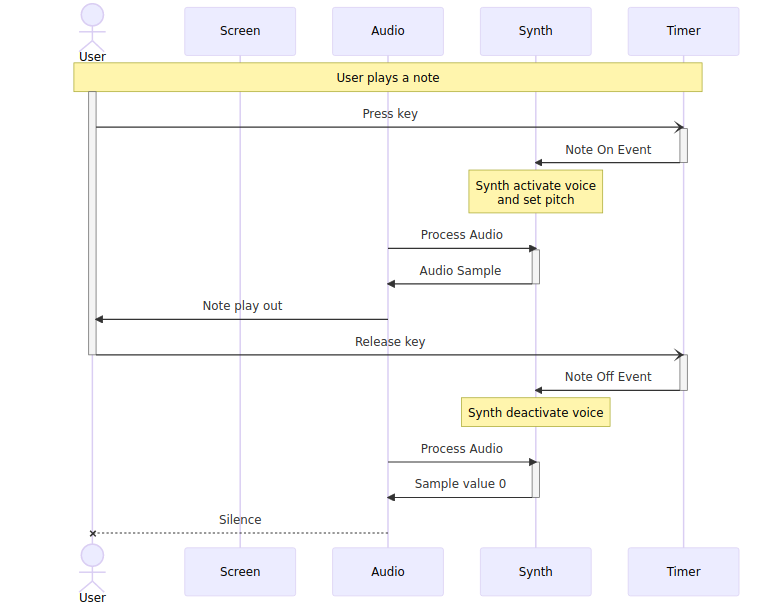
\includegraphics[width=.7\linewidth]{play_note_sequence}
		\caption{A sequence diagram of the interaction of the five main actors. The most common scenario is the user playing notes on the keyboard. The timer interrupt detects the MIDI message from the keyboard and triggers a \textit{note on} event for the synth. The synth responds by activating one of its voices and setting the voice's pitch according to the note on event. Next time the audio interrupt occurs, the synth will generate and return an audio sample from that voice. The audio interrupt puts the sample into the DAC buffer which plays out the speakers for the user. Audio will continue to be generated and played to the user until the key is released on the keyboard. The timer triggers a \textit{note off} event, telling the synth to deactivate the voice. Next time the audio interrupt occurs, the synth will return a zero valued sampled which results in silence for the user}
	\end{figure}
	
	Keeping these actors in mind, we can now begin to understand how the synth, timer interrupt and audio interrupt work together.
	
\subsection{The Synth and Its Modular Components}
	\paragraph{This section is a noncomprehensive explanation of the fundamental components that make up the audio processing pipeline} It is intended to provide an explanation sufficient to read and understand the source code. It should also provide sufficient information to be able to write your own implementation. Every synth needs to start with some kind of signal, so the first component to address is the oscillator.
	
	\subsubsection{Oscillators}
	\paragraph{The oscillator module is the very first component in the processing chain} This module is a class with just a few attributes: The oscillator frequency, n enum representing what kind of function it generates, a variable to track the phase of the function cycle, and delta variable for how much the phase should be incremented to produce samples at the set frequency. There are a few methods: set\_frequency, set\_waveform and get\_sample. 
		
	\paragraph{The get\_sample method is the core of the oscillator class} It generates samples for the current pitch and configured function. When the get\_sample method is called the sample is generated using the oscillator function with the phase variable as its input. After the sample is generated, the phase variable is incremented by the delta variable to prepare for the next sample. If phase exceeds the value of \( 2\pi \), the function's phase is complete and \( 2\pi \) is subtracted from phase variable to start the phase over. The generated sample is then returned as an output. Below is a sequence chart illustrating this process with the oscillator generating sin wave samples. The samples are used by the audio interrupt place in the DAC's output buffer for playback.\cite{farnell_2010}
	
	\begin{wrapfigure}{l}{.75\textwidth}
		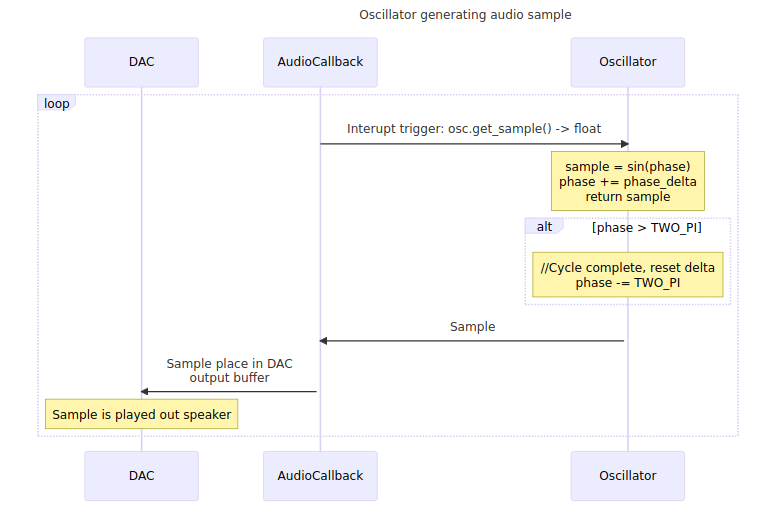
\includegraphics[width=\linewidth]{oscillator_sequence_diagram}
		\caption{Oscillator sequence diagram needs to be exported}
		\centering
	\end{wrapfigure}
	
	\paragraph{The phase and delta variables:} Mentioned previously, the delta variable (hereafter phase\_delta, the name of the oscillator classes member name) is a calculated value used to increment the phase. The value of phase\_delta is necessary to generate samples at the desired pitch.
	\paragraph{So how on earth do we calculate this magic phase\_delta?} Lets start simple, to generate a sin wave at 1hz with a sample rate of 44.1kz, we simply need to divide \( 2\pi \) by 44100 to get the phase delta. Phase is initialized to zero and phase\_delta is calulated with the function \( 2\pi/44100 \). Every time the audio callback occurs, the oscillator will return the value of \( sin(phase) \) and then increment phase by phase\_delta. After one second of time has passed, the audio callback will have triggered 44,100 times, phase\_delta will have been added to phase 44,100 times and phase will be equal to \( 2\pi \) completing one cycle, and a 1hz sin wave will have been played out the speaker. 
	
	\paragraph{Okay, well cool, but humans can't hear a 1hz sin wave and music is most enjoyable when it's audible} Let's make some noise we can hear: To change the pitch, we only need to multiply the 1hz phase\_delta by our desired frequency, so the formula for calculating the phase delta of your desired pitch is \( 2\pi/44100 * frequency \). \textit{Note: 44100 is not a hard and fast number. It is just the sample rate of the DAC. If the DAC is configured to use a higher sample rate like 96khz, then 44100 would be substituted with 96000. So the generic formula to calculate phase\_delta is \( 2\pi/sample_rate * frequency \). Note: The sample rate of the DAC and the sample rate used to calculate the phase\_delta \textbf{must} match or the pitch will be off} Okay, so going back to making music: If we want our oscillator pitch to be 100hz, our calculated phase\_delta will be \( 2\pi/44100 * 100.0\). This phase delta will cause the oscillator function to cycle 100 times in a second. Pretty simple. All this behavior is contained in the set\_pitch method in the Oscillator class. So now we have everything we need to generate sin wave samples at any pitch.
	
	\paragraph{"What about other waveforms? Sin waves are boring!"} Totally. Sin waves lack harmonic complexity and will generally produce very smooth and mellow tones. Let's talk about that function enum I mentioned before. The Oscillator class has an enum called WaveForm to indicate what \textit{kind} of oscillator it is (i.e. what function does it use). The oscillator WaveForm enum is set with the set\_waveform method. If the waveform is changed, the next time get\_sample is called by the audio callback, the function matching the new configured WaveForm will be used and generate a sample from your fancy new harmonically rich waveform. \cite{downey_2016} Beautiful! 
	
	\paragraph{So what kind of functions are we using here?} Besides the sin wave, all the classic wave forms are present: Sawtooth, Square, Triangle and White Noise. The square wave just an on/off function where 1.0 is returned the first half of the phase and -1.0 is returned during the second half. The sawtooth save is a function that starts the phase at -1.0 and ramps gradually to 1.0 at the end of the phase. The triangle resembles a sin wave but with a linear form instead of a curve giving it a triangular shape. White Noise is generated with a pseudo-random number generator. \cite{tagi_2019} The snippet below is a good start for understanding the oscillators different waveform functions. See Oscillator.cpp for the full source.
	
	
	\begin{minted}{c}
//Oscillator.cpp
float Oscillator::get_sample()
{
	switch (_waveform)
	{
		//Plain old sin wave. Simple and easy to generate
		case WaveForm::Sin: {
			sample = sinf(_phase);
			break;
		}
		//A triangle wave!. It's like a sin wave but pointy! That's neat.
		case WaveForm::Tri: {
			t   = -1.0f + (2.0f * _phase * TWO_PI_RECIP);
			sample = 2.0f * (fabsf(t) - 0.5f);
			break;
		}
		//Sawtooth. Sharp and full of harmonics that make it fat and sassy
		case WaveForm::Saw: {
			sample = ((_phase * TWO_PI_RECIP * 2.0f) * -1.0f) * -1.0f;
			break;
		}
		//The good old square wave. The classic sound of the 8-bit video game era
		//Chock full of vitamins and harmonic flavor!
		case WaveForm::Square: {
			sample = (_phase < _half_cycle) ? 1.0f: -1.0f;
			break;
		}
		//TV static. For noisy instruments like drums and sound effects
		case WaveForm::WhiteNoise: {
			sample = noise.process();
			break;
		}
	}
}
	\end{minted}

	\paragraph{"So I've got this oscillator. How do I control I start making music now?"} To control the oscillator, the timer interrupt listens for MIDI events on the UART line. When a note on messages arrive, the MIDI message is parsed to get the 7-bit number that contains the pitch of the note. This number can be accurately converted to the frequency value. This frequency can be passed to the set\_pitch method. However, an oscillator is pretty dumb. Once the pitch is set, it will play forever if no one tells it to shut up. As a workaround, when a note off message is received by the timer interrupt callback, you can set the pitch to zero hz to silence it. You can now use a MIDI keyboard to play pitches and turn them on and off. The system in this configuration is limited to one note at a time. The Voice component fixes this problem.
	
	\subsubsection{Voices}
	\paragraph{In the world of synthesizers, a single discrete note playing a certain pitch is called a voice} A voice is a structure that contains at least one oscillator of its own. A synth with two voices can play two pitches at once: the oscillator(s) in the first voice are responsible for generating the samples for one pitch and the oscillators of the second voice are responsible for the other pitch. The Voice module in this project has this functionality and more.
	
	\paragraph{The Voice module is an aggregation of two separate oscillator class instances}. The Voice module has a method called set\_pitch and get\_sample just like the oscillator module. The set\_pitch method sets the pitch of its respective oscillators. The get\_sample method gets samples from both oscillators, adds them together and returns the aggregated sample. There is a separate gain parameter for each oscillator to control the gain ratio between the two oscillators. The oscillators can be configured with any fundamental waveforms such as sawtooth or triangle. This allows the user to generate a variety of new hybrid wave forms. The voice class can optionally configure a pitch offset to the second oscillator; another common synth feature in synthesizers. By detuning one oscillator from another, you can generate even more complex waveforms with frequency beating, added intensity, or even complete dissonance if desired. Lets take a closer look at this Voice class.
	
	\begin{figure}[H]
		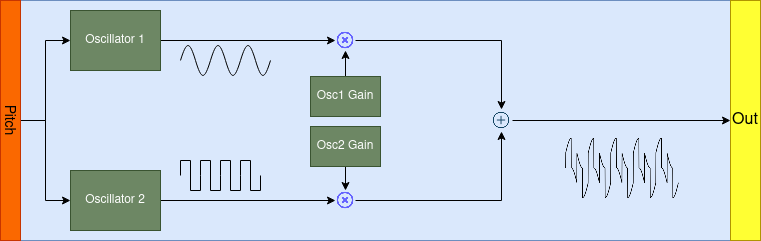
\includegraphics[width=\linewidth]{simple_voice}
		\caption{This example shows a voice with a sin wave oscillator and square wave oscillator. They each are attenuated by their own gain and then summed together to form a hybrid waveform that is returned by the voice}
		\centering
	\end{figure}
	
	\paragraph{In order to support polyphony, the pipeline needs a collection of Voice components and structure to manage them} A class called Synth represents the audio pipeline at its highest level. The Synth class owns a primitive array of Voice instances called \textit{voices}. The voices array holds eight voices instances more may be allocated. Eight seems to reach the upper limits of the needs of most musicians. With the voice class implemented, the pitch of the oscillators is not set directly by the timer interrupt as mentioned previously. Now, the timer interrupt sends MIDI note on and note off events directly to the synth class, which calls set\_pitch on a voice. The voice in turn will directly set the oscillator pitch.
	
	\paragraph{When note on messages are received, it loops through the array of voices until it finds a voice that is not currently active (i.e. playing a note)} Just \textit{how} the synth determines if a voice is currently active will be covered in the next section. Once the synth finds an inactive voice, it sets the voice's pitch according to the MIDI event and marks it as active. Marking a voice as active informs the synth which voices it should get samples from when an audio callback occurs. When note off events occur, the synth will loop through the voices once again until it finds the active voice with the matching pitch. It then sets the voice as inactive. Voices that are inactive will be skipped when the synth loops through the voice array during the audio callback. With this functionality in place, multiple notes can now be played at once, with the voices turning on and off as keys are pressed down and let up. If there is a time when a user pushes down more keys than there are voices, the note that has been active the longest will be deactivated and used to play the new note. This means the old pitch will be dropped from playback and replaced with the new one. This is a common policy for handling these situations in synthesizers.
	
	\begin{figure}[H]
		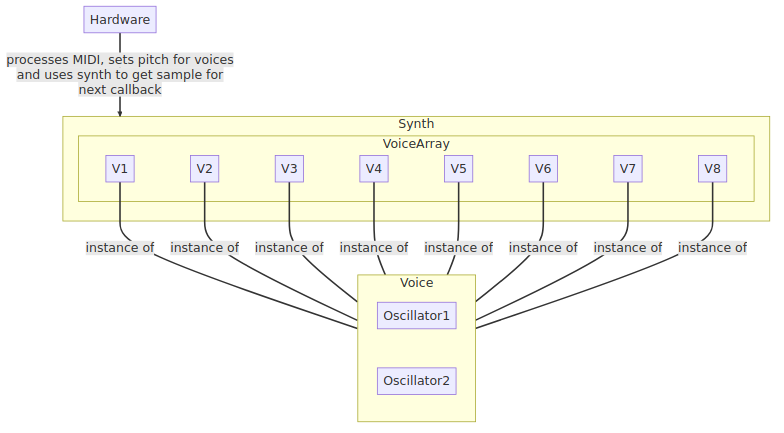
\includegraphics[width=\linewidth]{voice_graph_diagram}
		\caption{At this point in the system, the software architecture looks like this}
		\centering
	\end{figure}
	
	With voices and the synth class added to the architecture, the system is now officially a polyphonic synthesizer. To learn more, see Synth.cpp, Voice.cpp and Oscillator.cpp. The next component to address is the Envelope module.


	\subsubsection{Envelopes}
	
	\begin{wrapfigure}{l}{.5\textwidth}
		\centering
		\caption{The states of the envelope and the events that trigger phase transitions}
		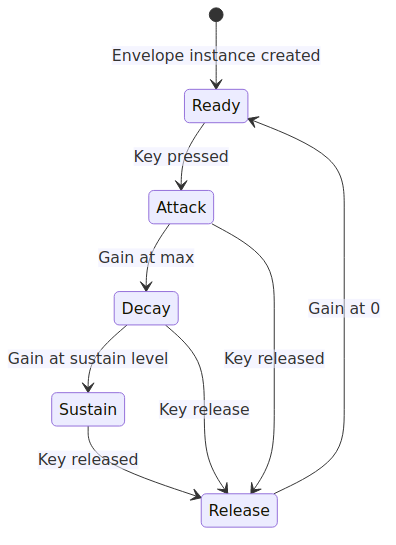
\includegraphics[width=.8\linewidth]{envelope_state_diagram}
	\end{wrapfigure}
	
	\paragraph{Musical instruments get louder and quieter over time in different ways}. A percussive instrument like a drum or piano will instantly play at maximum volume. The loudness will diminish over time depending on the instrument. A bell, when struck, will ring out for a long time unless the player mutes the bell. A snare drum will go quiet almost immediately after it reaches its maximum volume. Conversely, a violin can increase in volume fast or slow and can play at the same volume indefinitely. Synthesizers have a way of emulating volume dynamics with an \textbf{amp envelope}. Before jumping into the Amp Envelope, a quick explanation of envelopes is needed. 
	
	\paragraph{Envelopes are a multiphase signals that are used to modulate other signals over time} They commonly have four phases wherein the signal gain increases and decreases. These phases are known as Attack, Decay, Sustain, and Release.
	
	\textbf{Attack} is the first phase of the envelope. During the attack phase, the signal starts at 0 and ramps up to its maximum gain of 1.0. Attack represents \textit{how long} it takes for the gain to reach max. By pressing down on the keyboard, the envelope becomes active and transfers into the attack phase.
	
	The \textbf{Decay} phase occurs immediately after the attack phase. During the decay phase, the signal gain decreases until it reaches the configured sustain value. Similair to attack, the decay phase indicates \textit{how long} it takes for the gain to decrease sustain.
	
	The \textbf{Sustain} phase occurs immediately after the decay phase. During the sustain phase, the signal stays the same. Unlike attack and sustain, sustain does not relate to time, but simply the gain that the signal will decrease to after the attack phase is complete. As long as the note is held down on the keyboard, the envelope will remain in the sustain phase indefinitely.
	
	The \textbf{Release} phase occurs immediately after the key is released on the keyboard and is the final phase. The envelope can enter the release phase from any of the previously mentioned phases. Release refers to how long it takes for the envelope gain to return to 0 after the note is released. \cite{hass_2021}
	
	\paragraph{An amp envelope refers to when the volume of a voice is modulated by the signal gain of an envelope} Multiplying a voice's output gain by the amp envelope's signal results in the voice growing and diminishing in volume according to the phase of the envelope. This is how the synthesizer emulates the volume dynamics of many instruments. In a polyphonic synthesizer, every Voice must have its own amp envelope so that each note can grow and diminish independently of each other. The figure below shows the envelope signal and the effect it has on an oscillator when applied to the output gain. An envelope is triggered by a note on event. 
	
	\begin{wrapfigure}{r}{.5\textwidth}
		\centering
		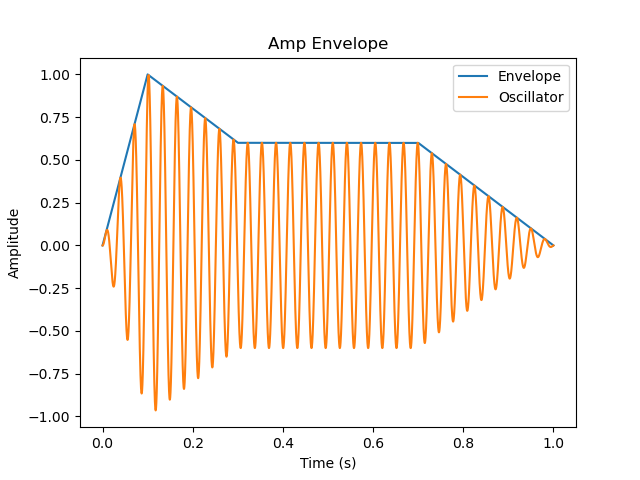
\includegraphics[width=.8\linewidth]{amp_envelope_visual}
		\caption{Graph of the amp envelope in action}
	\end{wrapfigure}
	
	\paragraph{The Envelope module is implemented as a state machine to represent the four phases of an envelope} In addition to the four previously mentioned phases, there is a state specific to this implementation called Ready. The ready state indicates that the envelope is currently inactive. Since every Voice in the synth has its own envelope, it uses voice's envelope state as an intuitive way to know if it is inactive. If a voice's amp envelope state is "ready", the voice is available to play a note. 
	
	\paragraph{The Envelope is designed to change its signal every time a method named \textit{process} is called}. In the process method, the gain is incremented or decremented by a certain amount until the gain reaches limit indicating the end of the phase. The envelope then transitions to the next phase. The amount by which the gain should be incremented is specific to the configuration of each phase. Since an envelope does not produce sound, the Envelope process method does not need to be run during the audio callback. The resolution of an envelope signal does not need to be so high in order to be effective. The much slower hardware timer takes on the duty of calling the envelope process method.
	
	\paragraph{So how do we calculate the increment value for a phase?} We take the difference of the gain value at the beginning of its phase and the gain value of the end its phase. We then divide the difference by the phase's time with respect to the timer callback frequency. For example, during the attack phase, the envelope gain starts at 0.0 and ramps up to 1.0. In this case, the difference between the start and end gain is 1.0. If the attack time is 300ms and the interrupt frequency is 1000hz, the attack increment is \( 1.0/(1000*.3)=0.00333 \) Incrementing by this value with every timer interupt will result in the envelope gain reaching 1.0 in 300ms. The rest of the phases can be calculated in a similar way. See the full Envelope class source for more details.
	
	\begin{minted}{c}
//Envelope.h
class Envelope {
	public:
	
	//State machine enum for tracking what phase the envelope is in.
	enum Phase {
		ATTACK,
		DECAY,
		SUSTAIN,
		RELEASE,
		READY 
	};
	
	float val = 0.0; //the current signal gain of the envelope
	Phase phase = Phase::READY;
	float process(); //called periodically by timer event callback to advance
	//the gain according to envelope phase state
	void note_on(); //Kicks of the envelope by settings its phase from ready to attack
	void note_off(); //Note off events will set the envelope to the release phase
	void reset(); //After release phase is completed or a new note must be played and all
	//voices are occupied, the envelope must be reset.
};
	\end{minted}
	
	\begin{minted}{c}
//From Voice.cpp: Shows the voice getting the next sample from its oscillators
//and multiplying the sample by the amp envelope's signal gain to attenuate
//the final sample before it is returned to the synth
float Voice::get_sample()
{   
	//samples from individual oscillators are attenuated by their configured gain
	float sample1 = (_osc1.get_sample() * _osc1_amp);
	float sample2 = (_osc2.get_sample() * _osc2_amp);
	return (sample1 + sample2) * amp_env.val;
}

//From Synth.cpp: Show the ProcessAudio function of Synth. While looping through
//the voices, if an voice amp envelope phase is in a ready state, it means the 
//voice is not active and should be skipped
float Synth::ProcessAudio() {
float sample = 0.0;
for(uint8_t i = 0; i < NUM_VOICES; i++) {
	if(_voices[i].amp_env.phase != Envelope::Phase::READY) {
		sample += _voices[i].get_sample();
	}
}
	\end{minted}

	\begin{figure}[H]
		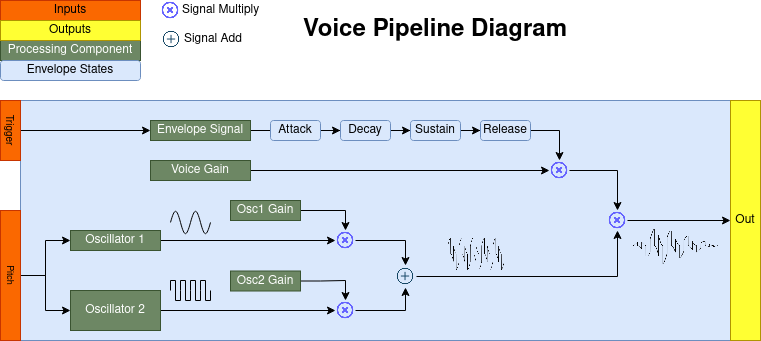
\includegraphics[width=\linewidth]{Voice_Pipeline_Diagram}
		\caption{The final Voice component is a mini pipeline itself, processing digital audio data through many functions with the envelope being used as a data source to modify pipeline functions in real time.}
		\centering
	\end{figure}
	
	
	\paragraph{The introduction of envelopes shows how deep the modular nature of synthesizers is} They are not a part in the linear chain of the audio processing pipeline. They are functions running parallel, injecting inputs into other modules. Envelopes can be used generically to modulate any kind of signal such as volume, filter frequency cutoff, or even the gain of an audio effect like reverb or distortion. The application of envelopes is limited to your imagination making them a powerful tool in audio synthesis. The same implementation of the envelope can be reused anywhere in the Synth class. Two more envelopes are planned for the Synth class with the added feature of routing their signals to arbitrary data members within the class. Where the envelope signals are applied can be configured through the hardware menu interface. With Voices and Envelopes implemented, we now have polyphony and volume dynamics. The remaining component to bring the synth to life is filters.

	\subsubsection{Filters}
	\paragraph{Up until this point, the control of the harmonic qualities of synth was fairly limited} The fundamental waveforms can be combined, mixed, and have their pitch altered to create harmonically rich signals. But the subtractive aspect of this subtractive synthesizer is conspicuously missing. Filters make up the subtractive nature of the system. They allow the user to selectively chop frequency bands from the final signal to emulate real-life instruments.\cite{welsh_2006} An synth audio filter typically has two main parameters: Frequency cutoff and resonance. Frequency cutoff (or just cutoff) determines the point where the filter begins cut out parts of the frequency spectrum. Resonance is a gain boost that can be applied around the cutoff frequency to boost a certain frequency band. \cite{musictech}
	
	\paragraph{The most common filters used in subtractive synthesis are low pass, high pass, and band pass filters} Applying a low pass filter to a signal has the effect of removing the more harsh upper harmonic frequencies making the signal more mellow and deep. This type of filter is effective in producing sounds like a bass guitar, bass drum, or cello. Applying a high pass filter will cut out the low frequencies in the signal. This is useful for creating a lead instrument intended to cut through the spectrum without sounding muddy from the lower range of frequencies. Usually, a high pass filter will be used to produce sounds like a flute, violin, or snare drum. A band pass filter is a combination of low and high pass filters. Both the high and low ends of the spectrum are removed leaving a small frequency band in the middle range. The system implements a Filter class that can be subclassed into the different types of filters depending on the desired frequency response. \cite{hass_2021} 
	
	\paragraph{My implementation of the Filtering is fairly simple: it uses a second-order difference equation} The difference equation is a type of discrete time-system that relates an output sample y[n] to its previous sample y[n-1] and y[n-2]. It applies also to input samples, relating input sample x[n] to x[n-1] and x[n-2]. When applied to an audio pipeline, it allows filtering to be performed on a discrete time signal within in a continous time domain.\cite{stanford_2007} The second-order difference equation is as follows: 
	
	\scalebox{1.3}{\( y[n] = (b0x[n] + b1x[n-1] + b2x[n-2] - a1y[n-1] - a2y[n-2]) \)}
	
	\paragraph{The variable y represents filtered output values and x represents unfiltered input values} The variables b0, b1, and b2 are known as feed forward coefficients. The variables a1 and a2 are known as feedback coefficients. The second-order difference equation is used to implement an \textit{infinite impule response}. The equation can be extended to perform all the needed functionality of our filter:
	
	\scalebox{1.3}{\( y[n] = \frac{b0}{a0}x[n] + \frac{b1}{a0}x[n-1] + \frac{b2}{a0}x[n-2] - \frac{a1}{a0}y[n-1] - \frac{a2}{a0}y[n-2] \)}
	
	\paragraph{In the updated function, we divide each of the feedback and feed forward coefficients by a third coefficent a0 which is known as the normalization coefficient} The normalization coefficient's function is to normalize the final output sample to unity gain and is calculated based off the filters resonance factor. The higher the resonance factor of the filter, the more a0 will boost the gain around the cutoff frequency. If you're as unfamiliar with DSP as I was when I started and you feel lost, you're in good company. It took many hours of staring and beard stroking for this to finally start clicking. I still feel my brain go fuzzy when I think about it. This section is packed with citations of textbooks on filters provided by several universities for free and can be read online for more information. \cite{lacamera_2020}
	
	\paragraph{"Okay. I believe you when you say this works. Now just where on earth did you get these coefficients?"} Because we are attempting to digitally emulate a filter that operates in the continuous time domain, we need to generate filter coefficients that will approximate the frequency response discrete time domain. A method known as bilinear transform is used to map a transfer function (in this case the filter frequency response) from the continuous time domain to a discrete time domain. By applying the bilinear transform, we can take approximate the coefficients necessary to perform the second order difference equation filter. The equation for bilinear transform is as follows: \cite{stanford_2007} 
	
	\scalebox{1.3}{\( s=c\frac{(1-z^{-1})}{(1+z^{-1})} \)}
	
	\paragraph{In the equation, s is a complex variable representing the filter coefficient in the continuous time domain} The variable z represents a discrete time transfer function which in our case is our filter cutoff frequency. The variable c is an arbitrary constant that is used to accurately map an analog frequency to a digital frequency. We can substitute z with a discrete time transfer function of the  filter cutoff frequency. The value of c is set to \( \frac{2}{T} \) where T is the sample rate. Evaluating the bilinear transfer will give us the coefficients we need for the difference equation filter. Below is a snippet of the coefficient calculation in action with extra comments explaining what is going on. The math for calculating the coefficients can quickly explode into long expressions. So some simplifications are made to keep thing easy on the eyes and brain. To get the dirty details, see the sources.
	
%	\paragraph{You may be wondering why most of the coefficients are just the first feed forward and feedback coefficients with extra arithmetic operations} The reason is that the first coefficient is just a constant that represents the frequency response of the filter. All the coefficients following are just minor attenuations or complete copies of the first in order to  The first coefficient is divided by two since the filter damping effect should be the weakest right at the cutoff frequency. The second is strongest to provide the greatest dampening effect. The third coefficient b2 is identical to the first, because by this point, the sample effected by b2 has already been significantly dampened by b0 and b1 so b2 will just do it a little bit more.
	
%	The alpha portion of the filter represents how steep the attenuation of the signal is around the cutoff frequency of the filter. Resonance plays a part in the alpha coefficients as the resonance will factor into how much gain is applied around the cutoff frequency of the filter. Following is my code implementation of the low and high pass filters in my project with a sequence diagram to help visualize the flow of data through the filter and how previously generated values are stored for use on the next filter cycle.
	
	\begin{minted}{c}
//Filter.h
class Filter {
	public:
	Filter(float sampleRate, float cutoffFrequency, float q);
	virtual float process(float input) = 0;
	void set_cutoff(uint32_t freq_hz);
	void set_resonance(uint32_t gain);
	virtual void update_coefs() = 0;
	
	float cutoffFreq;
	float resonance;
	
	private:
	float sampleRate;
	float b0, b1, b2, a0, a1, a2; //These private members are the coefficients
	//used in a difference equation during processing. More on that later.
	
	/*
	These members contain inputs and filtered outputs
	from previous process cycles. x1 and x2 are the original input samples
	from the two previous process events. y1 and y2 are the filtered outputs
	from the previous two process events. They must be used in the difference
	equation
	*/
	float x1, x2, y1, y2;
};



//This snippet of the second-order difference equation shows how
//the output is generated based on previous inputs. Each time process
//is called, the input and output values and shifted over two be processed
//with the next coefficients on the following process cycle. input becomes
//x1, x1 becomes x2, etc. Each input and output will be multiplied by each
//coefficient and incorporated into the final filtered sample which is the
//function of the difference equation.
float LowPassFilter::process(float input) {
	float output = b0 / a0 * input + b1 / a0 * x1 + b2 / a0 * x2
	- a1 / a0 * y1 - a2 / a0 * y2;
	
	x2 = x1;
	x1 = input;
	y2 = y1;
	y1 = output;
	
	return output;
}

void LowPassFilter::update_coefs() {
	//Normalized cutoff frequency in radians per sample in digital domain.
	float cutoff_norm = 2.0f * M_PI * cutoffFreq / sampleRate;
	
	//Applying cosin function to the normalized cutoff frequency to simplify
	//the expressions for the bilinear transform
	float cutoff_cos = std::cos(cutoff_norm);
	
	//freq_response_shape is refers to the shape of the frequency response
	//in the filter as well as resonance boost around the cutoff frequency
	float freq_response_shape = std::sin(cutoff_norm) / (2.0f * resonance);
	
	//A couple of steps in one here performing the bilinear transform
	//We perform the bilinear transform by substituting the continuous time
	//transfer function of the frequency cutoff to a transfer function of
	//the frequency response in discrete time domain
	b0 = (1.0f - cutoff_cos) / 2.0f;
	b1 = 1.0f - cutoff_cos;
	b2 = (1.0f - cutoff_cos) / 2.0f;
	a0 = 1.0f + freq_response_shape;
	a1 = -2.0f * cutoff_cos;
	a2 = 1.0f - freq_response_shape;
}
	\end{minted}
	
	\paragraph{With filters added to the mix, the synth is now subtractive and has endless potential to create new sounds} Many components remain to be implemented to the signal processing chain, like delay, reverb and overdrive effects. But the core system is in place and highly configurable. Next, I will explain the high level architecture of the hardware and how user interacts with it to drive the synth.
%	
%\subsection{Hardware Platform}
%	\paragraph{A big decision in implementing this project was choosing the right microcontroller platform} I considered several options but settled on a popular and relatively new audio development ecosystem by Electro-Smith known as Daisy. Daisy is an Arm Cortex-M7 based development board that provides all the necessary processing power and peripherals necessary for audio processing. Daisy's core processor clocks at 480Mz and includeds extremely high-resolution digital-to-analog converter (DAC). In addition to the DAC, it supports the expected communication protocols such as I2C, UART, USB, Timers, etc. The biggest benefit to choosing Daisy as my platform was Electro-Smith's libDaisy library. libDaisy acts as an abstraction on top of the standard HAL libraries for the Cortex M7 and is designed to relieve the user of complications with hardware set up so they can focus on audio development. \cite{electro-smith} This made Daisy an attractive option. Audio processing was a completely foreign domain in programming, and Daisy coupled with its easy to use HAL seemed like a promising option that would give me the time I need to learn the ropes of audio development.
%	
%	\begin{wrapfigure}{r}{.5\textwidth}
%		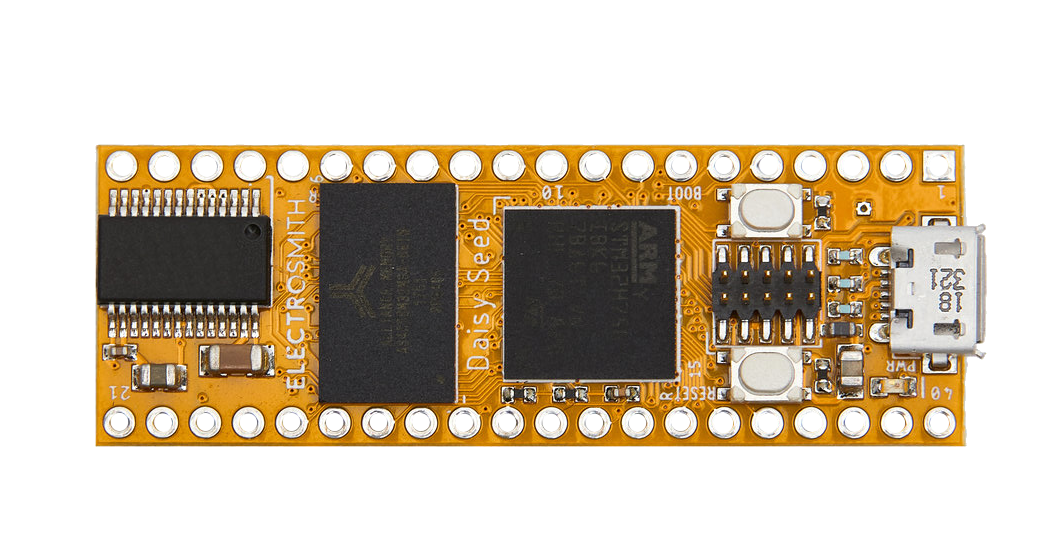
\includegraphics[width=\linewidth]{daisy_promo_pic}
%		\caption{Daisy Seed by Electro-Smith. The microcontroller platform for this project}
%		\centering
%	\end{wrapfigure}
%
%	\paragraph{Daisy seemed to be a great choice at the time} Within minutes of connecting Daisy to my machine, I was able to set up an audio callback. I used a random number generator to play white noise out the DAC. After a few minutes of soldering some wires to an audio jack and connecting them to the DAC pins, I could hear static playing out my headphones. Hello world! It was exhilarating to write only a few lines of code and hear it come to life after a few minutes. I felt very strongly that Daisy was the right choice. What I was not aware of was the relative newness of the platform. Daisy originally was a Kickstarter-funded project which received incredible amounts of success and support. The platform was designed with musicians in mind, and the developers put a lot of work into supporting much more user-friendly development languages and frameworks like MaxMSP, Puredata, and Arduino. This made the system highly accessible to musicians with little to know experience in audio development. These layers of abstraction seems to have some unintended side effects. It meant that a lot of time put into customer accessibility, and full support for utilizing all hardware to its fullest capabilities was put off and is still in current development.
%
%	\paragraph{My original vision for the project was, as the master's capstone prompt recommends, very ambitious} My goal was to implement a near clone of \textit{my} first synthesizer, the Korg microKorg. The microKorg is a small but very powerful analog synthesizer with a minimalist interface. It has a small array of buttons for selecting patches from bank, an array of multifunctional potentiometers and a small 3 digit 7 segment display. My project would be in a similar spirit but with a few minor change in hardware layout: it would not include a built in keyboard but would be a headless unit that could be used by plugging in any standard MIDI keyboard. It would include a more sophisticated display that could communicate more explicitly to the user. The microKorg is an industry standard powerhouse synth packed into a small and inexpensive form factor. My goal was ambitious to say the least. \cite{ward_2003} At one point, I did have a stretch goal in mind. If I finished all the audio components and fx, I would add a small array of buttons that would allow the user play some notes without needing to connect a keyboard. This can be seen in my original design drawing. I truly was a bright-eyed summer child when I first envisioned this project.

%	I will explain my implementation by first covering what I managed to complete. I will discuss the key components in the order they were implemented, and then have a small section cover the lesser features and a run down of the things I failed to complete.

\subsection{The Hardware Prototype}
	\subsubsection{MIDI}
	\paragraph{There is a 5-pin MIDI input circuit that allows the user to connect a standard MIDI cable between the MIDI output of a keyboard and the synthesizer} This functionality is plug-and-play. By plugging in the MIDI cable and powering on the device, the user can immediately start playing notes and music will play out headphones or a speaker  plugged into the 1/8" audio jack.
	
	\begin{wrapfigure}{l}{.5\textwidth}
		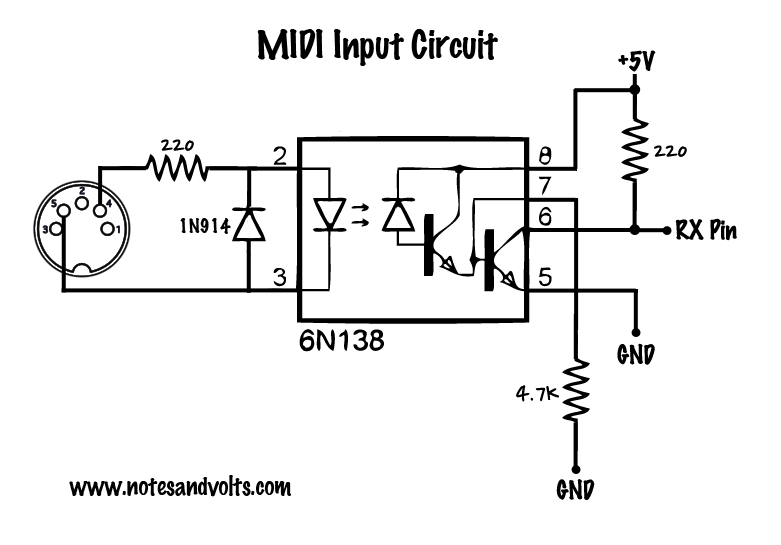
\includegraphics[width=8cm]{midi_optocoupler_circuit}
		\caption{The MIDI input optocoupler circuit}
		\centering
	\end{wrapfigure}

	\textbf{The MIDI circuit implements a standard of device safety for receiving incoming signals:} A device called an optocoupler (6N138) is the main player in the circuit. One side of the optocoupler receives incoming electrical signals from the MIDI input and converts it into an optical signal with an internal flashing diode. The other side senses the optical signal and converts it to an electrical signal that is safe for the device to read. This safety precaution is meant to handle cases where the connected keyboard is malfunctioning or outputting an electrical signal that is too high voltage for the pins on the MCU. If device failure occurs and the system is exposed to dangerous currents, the optocoupler will fry and the rest of the system remains protected. \cite{notesandvolts}
	
	\paragraph{After the oscillators were properly implemented, I added the MIDI message processing} I looked through some blog posts about consuming MIDI data through a UART connection and found the optocoupler circuit. I ordered the parts and got it working quick and easy. As data arrived on the UART line, I parsed the bytes into MIDI messages. MIDI note\_on messages were received when a note was pressed on the keyboard. MIDI note\_off messages were received when the key was released. Both message types contain a 7 bit number indicating the key that was pressed and a 7 bit number indicating the velocity (\textit{how hard} the key was pressed).\cite{huber_2007} When note\_on messages arrived, I converted the integers to the correct floating point frequency values and set the oscillators pitch. The oscillator would play the new pitch out the speakers. When note\_off messages arrived, the pitch of the oscillator was set to 0hz to silence the oscillator. At this point, I had the absolute bare minimum definition of a synthesizer. It could play a note sent from the keyboard, and the oscillator would respond by playing the correct pitch with its configured waveform. It could only play one note at a time and could not generate any signals more complex than the 5 basic oscillator functions, but nevertheless, it was a big step in the right direction. Adding polyphony and waveform mixing was the next logical step.	
	
	
	\subsubsection{Analog Potentiometers, Digital Rotary Encoder and Screen:}
	I ran with the design philosophy of the Korg microKorg and set up an array of 5 analog potentiometers. The potentiometers have control over various synth parameters. The parameters they effect are contextual, determined by the current internal state of the synthesizer. The internal state of the synthesizer is communicated to the user with a 20x4 character LCD screen that shows the user the current mutable context of the system. There is a main menu that displays a list of all the available menu context they can operate on. They can scroll through the main menu by turning the digital rotary encoder. The menu indicate which menu context is ready to be selected with an arrow symbol "<-". The user can then select the menu context by pushing down on the rotary encoder. They menu context will change to display the mutable parameters and the potentiometers will be mapped to the appropriate parameter values. Turning the turning the encoder knob will return them to the main menu and deactivate the potentiometers.


	\begin{figure}[H]
		\centering
		\begin{subfigure}{.5\textwidth}
			\centering
			\caption{The Main menu screen. User navigates by through options using the rotary encoder. No menu context is currently selected making potentiometers inactive}
			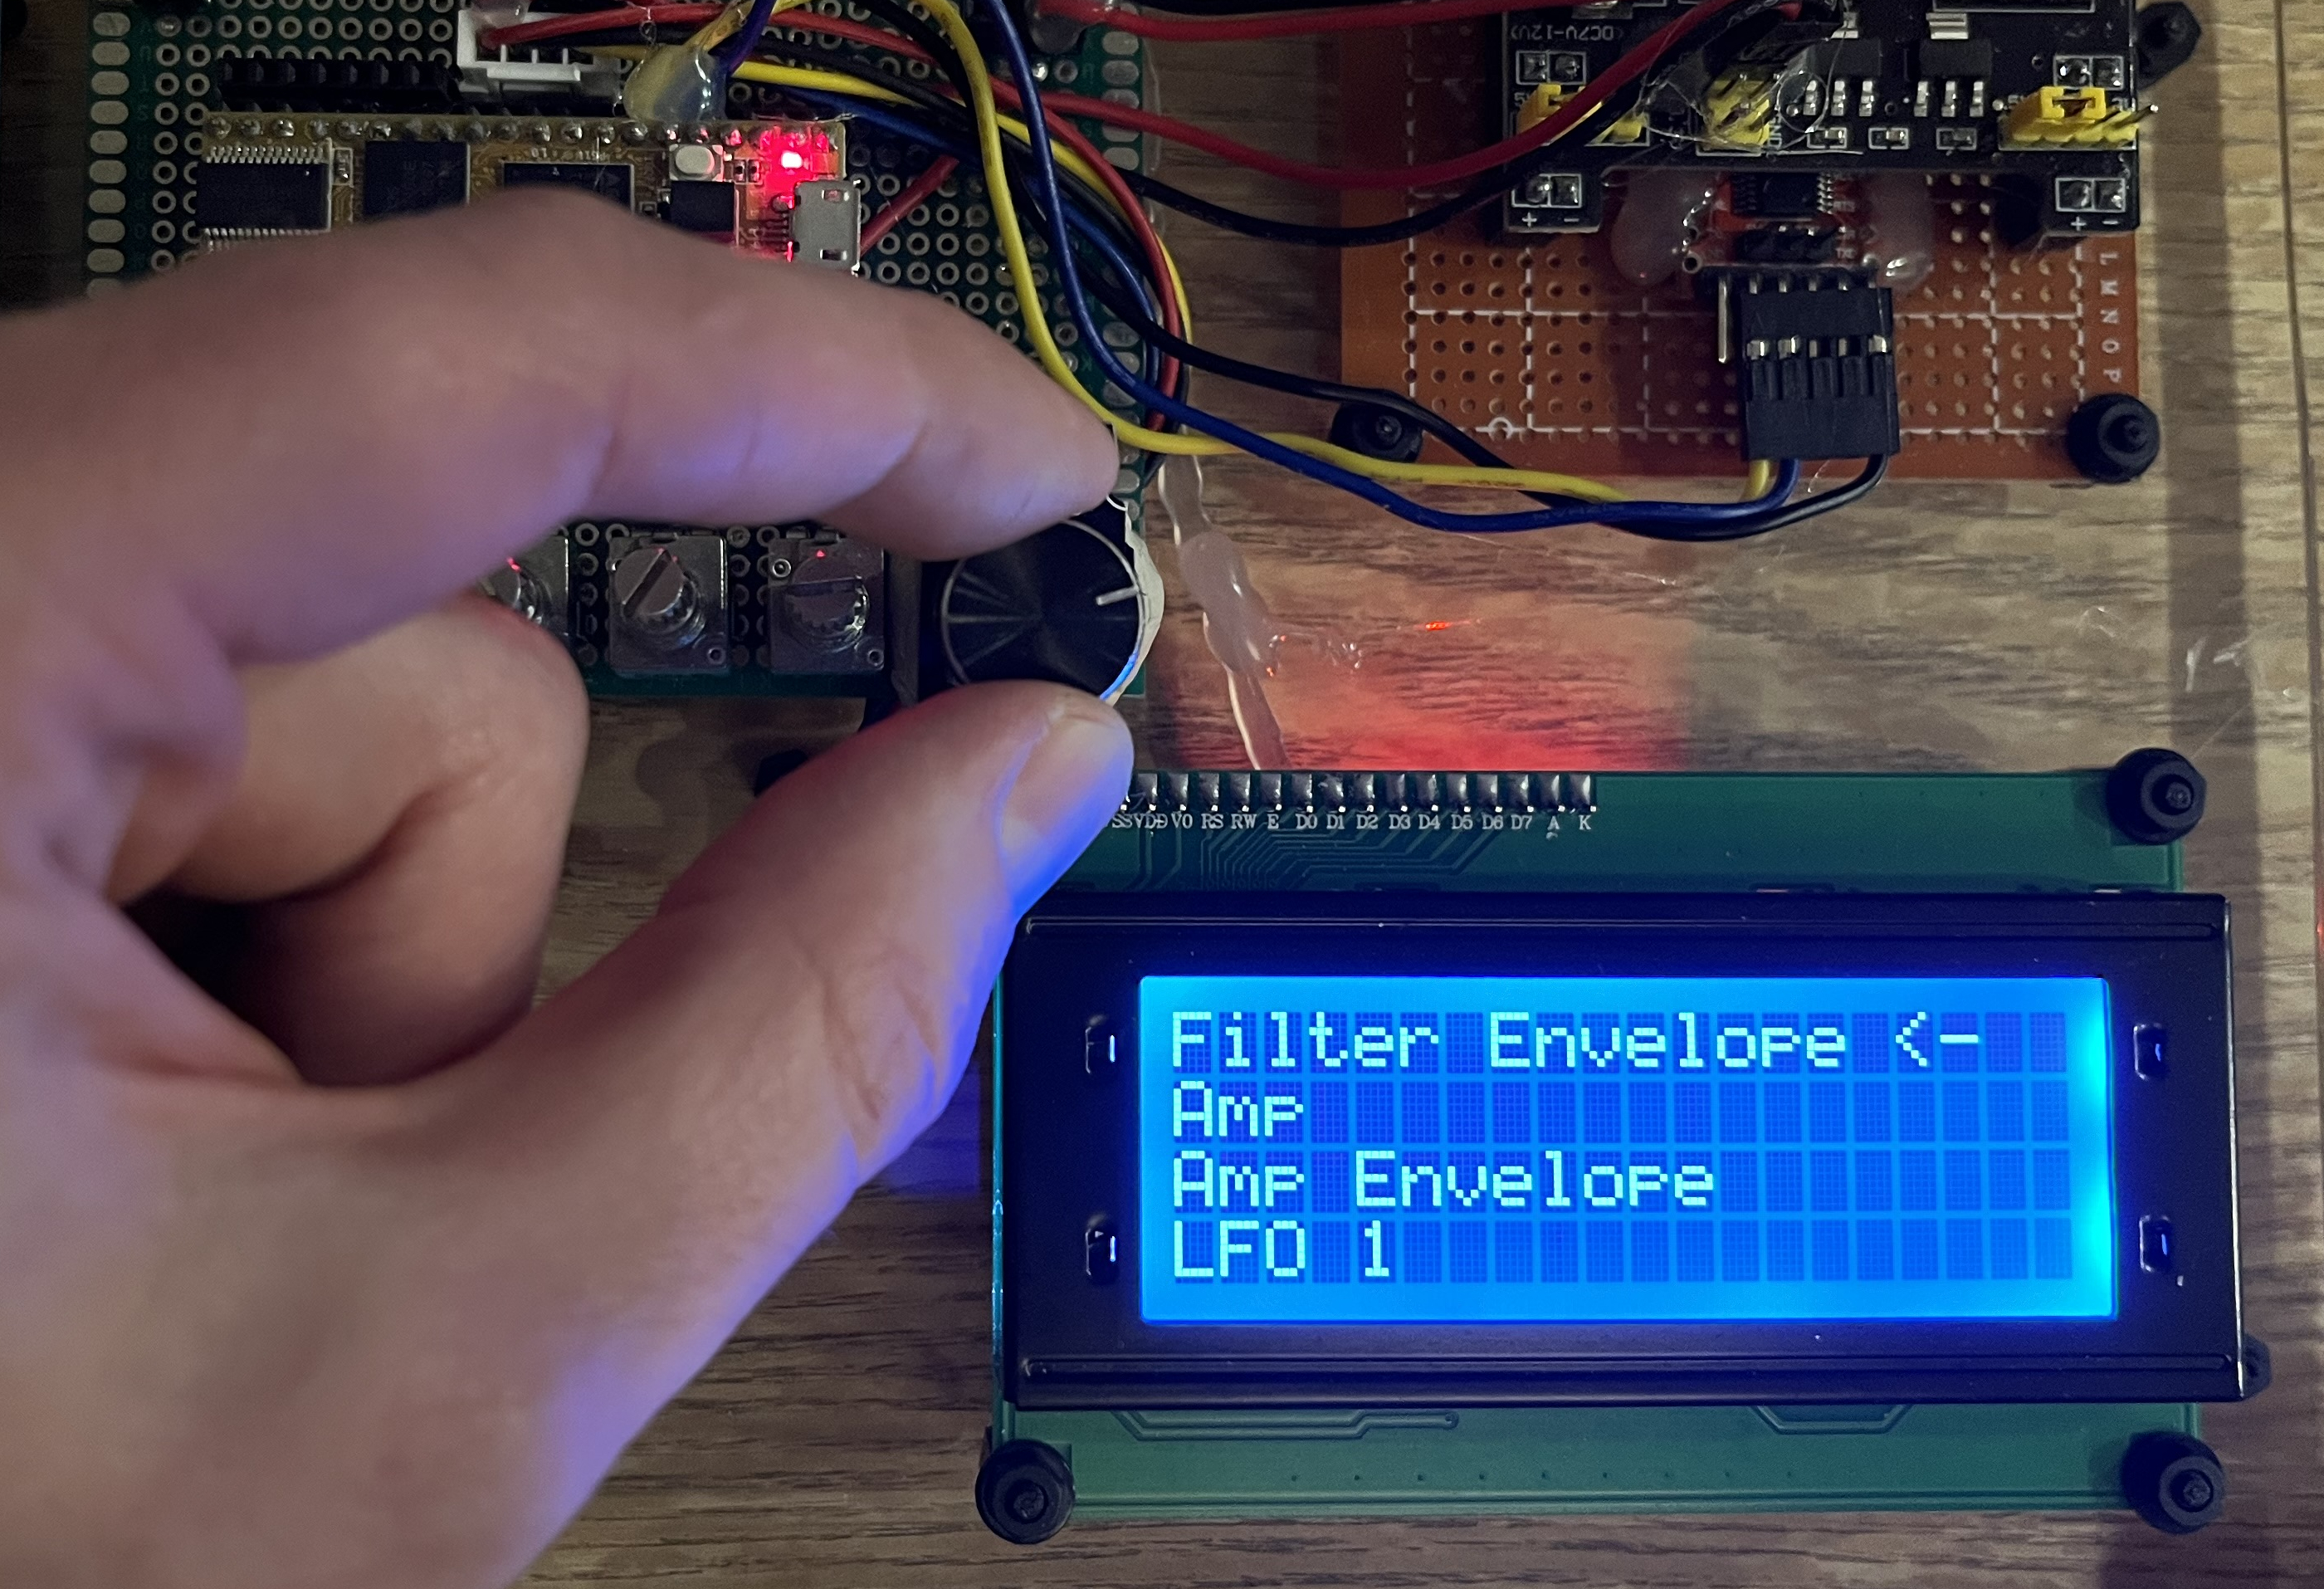
\includegraphics[width=.9\linewidth]{complete_synth_pics/menu_navigation}
			\label{fig:sub1}
		\end{subfigure}%
		\begin{subfigure}{.5\textwidth}
			\centering
			\caption{The oscillator context. Knobs 1-4 are mapped to the displayed parameters}
			\includegraphics[width=.9\linewidth]{complete_synth_pics/oscillator_context_small}
			\label{fig:sub2}
		\end{subfigure}
		\caption{Navigating the menus with the encoder and using the adaptive potentiometers to mutate system parameters}
		\label{fig:test}
	\end{figure}	

	For example, if the menu is displaying the oscillator control context, you can use the potentiometers to configure the oscillator waveforms and adjust pitch offset. If the menu was instead displaying the Amp Envelope control context, the knobs would be mapped to adjust the Attack, Decay, Sustain or Release parameters of the envelope. The parameter mapping also perform specific interpolations on the raw data values read from the potentiometers. Since some parameters are better controlled logarithmically, the integer value read from the knob can be converted to a float and scaled according to its required range. Some parameters only have a few discrete values. In these cases, the large values of the 16-bit numbers are instead mapped to the smaller ranges required to represent the discrete values of the parameter.

	\subsubsection{The rest of the hardware:}
	\textbf{Power:}
	The 20x4 LCD screen and the optocoupler on the MIDI input circuit require a 5v power supply, which Daisy does provide Yet another frustrating aspect of the Daisy platform since there is 5v power available on the USB jack. So I added a standard breadboard power supply to the circuit. It accepts a barrel jack input with voltages between 5v and 12v and steps the power down to 5v. This voltage is fed into the VIN pin on Daisy and is used to power the entire circuit and all its peripherals. A 1/8" inch stereo audio jack is connected to the left and right DAC pins on the MCU and outputs audio at line level gain out of the box without the need of an amplifier (a very nice feature). Finally, there is a USB to UART converter breakout board connected to a set of RX/TX UART pins on the MCU which allows two-way communication between an external computer and the synthesizer via a remote control GUI I wrote in Python.
	
	\textbf{Digital to Analog Converter (DAC):} 
	Daisy has a built-in high-resolution digital-to-analog converter. It is capable of outputting audio samples at rates up to 96khz and 24-bit depth. This resolution far exceedes the industry standard quality of 44.1khz and 16-bit depth for CDs. There are four DAC channels: two for stereo input and two for stereo output. In this project, I only use the stereo output as processing audio input is beyond the scope of this project.

	\textbf{UART, I2C, and 16-bit input ADC:}
	General purpose pins were configured to set up UART, I2C, and ADC communications Two separate UART lines were used for setting up MIDI input and plain serial communication for controlling the system remotely. The ADCs were used for reading the potentiometers. Some GPIO pins were used to read the digital rotary encoder for menu navigation. An I2C line is used to display characters to the LCD screen.

	\begin{figure}[H]
		\includegraphics[width=.8\linewidth]{complete_synth_pics/keyboard_and_synth_labeled}
		\caption{The entire synth hardware set up with labels}
		\centering
	\end{figure}

\subsection{Software Architecture}
	



\subsection{Pipeline Components}
	\paragraph{This section goes into depth about the various software components that make up the audio processing pipeline} I will address the software components in the order that they were implemented throughout the project. This will help to highlight the process of generating audio from the initial keyboard input to eventual output of the audio to a speaker. I will cover the topics of \textbf{Oscillators, Voices, Envelopes, and Filters} in depth as these are the critical components of the actual synthesis aspects of the project. I will only very briefly discuss other features in a few sentences as they have less to do with audio synthesis and more to do with overall system cohesion and functionality. \textit{See concepts for definitions and background info}
	
	\subsubsection{The "little big" software features}
	\paragraph{These are features that I would say are easily overlooked when they work, but utterly infuriating when they're broken} Some features were so important that they couldn't be ignored but sucked away a critical amount of time from the actual audio processing.

	\textbf{The LCD Screen:} I set up an I2C bus and wrote a driver to communicate with the LCD allowing me to quickly print menu information to the screen. This was a tediously long process with a lot of trial and error and sucked up about 2-3 weeks of my time. But it works very well and was critical in implementing the menu system.

	\textbf{The Hardware Timer:} I set up a hardware timer that triggered an interrupt service routine for reading peripherals. This effectively is a polling mechanism because of the lack of support for GPIO  in libDaisy. This timer callback would read the analog potentiometers, the rotary encoder, and the MIDI UART line and respond to any inputs on these peripherals. This timer was also used to advance the state of the amp envelope (See envelope section for details).
	
	\textbf{The Menu:} Running with the driver code for the LCD screen, I built up a class that will display the menu and its corresponding contexts. The Menu maintains a data structure of configurable parameters for the synthesizer such as oscillator waveforms and filters. The general purpose potentiometers adaptively manipulate menu parameters under the hood according to the currently selected menu context.
	
	\textbf{Remote Control GUI Application:} A simple GUI control panel app was written in Python using the QT framework to be to remotely change parameters without the need to physically interact with the synthesizer beyond simply playing keys on the keyboard to generate sound. This was accomplished using a secondary USB cable to communicate via USB Serial to tell the synth what parameters to change. This GUI also allows the user to save custom patches to a file on the host PC's disk, which can be loaded at will to instantly reconfigure the system according to the patch. This feature is still in development but is mostly complete with the ability to change a few parameters. The USB Serial driver provided by Daisy is susceptible to failure when too much data is sent down the line too quickly. Some more time is needed to determine how to make the app play nicely with the faulty serial driver.

\section{Conclusion}
	\subsection{Successes and completed features} 
	\paragraph{I accomplished to core requirement of my project:} Implement a real-time subtractive synthesizer from scratch on an embedded device. My system uses oscillators to generate tones with pitches based on user input from a generic MIDI keyboard. The tones are combined and processed through an amp envelope to add dynamics. The output from the envelope is processed through filters to carve frequencies out of the audio signal. The final processed audio signal is played out speakers or headphones which can be heard by the user in real-time without interrupts like pops or clicks in the audio. This here is a real working synthesizer; no ifs and or buts about it.
	
	\subsection{Total Failures}
	\paragraph{I did not manage to correctly implement some features into the system} Sometimes while developing the system, I made some critical mistakes that cost me valuable time.
	\begin{enumerate}
		\item I failed to add support for saving patch parameters to flash on the device itself. Bugs were encountered with libDaisy that made this too difficult to accomplish in my timeline.
		\item It took several attempts with weeks of effort to create a handmade circuit board to contain all my hardware components. My first attempt at laying all the electrical components on a circuit board was based on making flying wire harnesses that attach to all the human input peripherals. My thinking at the time was that making flying harnesses would make it easier to put the whole system into an enclosure. What resulted was a noisy mess of wires that made me feel physically ill when I looked at it.
		\begin{figure}[H]
			\includegraphics[width=.5\linewidth]{hardware_gore}
			\caption{Behold hardware gore: My first attempt at a prototype on perfboard}
			\centering
		\end{figure}
		\item In the process of adding an external power supply capable of providing power to the MIDI input circuit and LCD screen, I accidentally wired my power source into the wrong pin on the microcontroller. I fried the device, releasing the magic blue smoke. This isn't the first time I've done this and despite my efforts to not repeat the sins of the past, it happened. For a while, I had to move forward with development and adapt to not having a microcontroller while I waited for a new one to be delivered.
	\end{enumerate} 
	
	\subsection{Lesser Failures}
	\paragraph{Several optional features were planned for the system but had to be dropped for the sake of time} 
	\begin{enumerate}
		\item General purpose Envelopes to the system that the user could route to various components to be used for modulating arbitrary signals like filter cutoff, audio effect gain, oscillator pitch, etc.
		\item Low-Frequency Oscillators (LFOs). LFOs are non-audible oscillators that are used for arbitrary signal modulation similar to the previously mentioned general-purpose envelope. You can take the generated signal of the LFO and use it to modulate things like the pitch of an oscillator to add pitch vibrato. You can apply LFOs to filter cutoff to create filter "swishing" effects. You can apply it to the gain of the left and right audio outputs to create a panning effect between the left and right channels.\cite{paris_2022}
		\item Support for additional MIDI input messages were planned like the pitch and mod wheel devices often built into keyboards.
		\item An audio FX chain on the end of the pipeline to add effects like reverb, echo and distortion. These audio FX can add spatial features and additional audio coloring, expressiveness and complexity that users tend to enjoy playing with most.
	\end{enumerate}
	
	\subsection{Hindsight: "Choices" were made} 
	\subsubsection{The Daisy Platform:} Choosing to base my master's project on the promising platform of Daisy had serious consequences on development. Daisy was a very attractive option that promised a system that relive me of the more frustrating hardware complexities and make it easier to write audio processing software. The truth is, this is a new product. It focuses on implementing features to make development easier for hobbyists so they can make smaller audio FX processors and instruments. I would have been better off choosing a more mature audio-centric board from ST Microelectronics and using the tried and true STM32Cube IDE and setup the hardware myself.
	\subsubsection{Hardware Implementation:} Too much time was spent trying to migrate my project off of a breadboard and onto a permanent circuit board. I thought I knew enough of what I was doing that I could move my project off the breadboard and into a permanent enclosure without any intermediate steps or revisions. The flying harness prototype was a time vortex of disaster. After all that effort, what I had made was garbage and it now sits in a drawer. It's new function is to remind me to prototype incrementally and plan ahead.
	\subsubsection{Spaghetti Code and Tight Hardware Coupling:} As the system rapidly developed, some holes in previously developed features became more obvious as the system grew. These issues had to be ignored in favor of moving forward with development to meet the deadline. At times, refactoring software would create regressions that would cost even more time to fix. Some software refactoring and reorganization would help to make it faster and easier to add additional functionality to the system. In hindsight, I wish that I had designed the audio components to be more modular. If they had no hardware dependencies, I could easily test them out without the microcontroller and the synth system as a whole. Software fixtures could have been written to run unit tests on individual audio components. I believe this would have resulted in more rapid audio development first deploying and testing on my host machine without hardware in the loop. Once I was satisfied, the code could be integrated with the device firmware.
	\subsubsection{Performance Issues and Bottlenecks}
	Overall, there doesn't seem to be much of a bottleneck in the audio pipeline within my project. The synth is never late to deliver audio samples to the output DAC, so there are never any audio crackles or pops in the final audio played out the speakers. Many of the CPU clock cycles are spent just waiting for the audio and timer callbacks. The only major performance issue that currently persists is the noisiness of the potentiometers. Sometimes I feel like the potentiometers will get super noisy just by looking at them wrong. A software filter was written to smooth out the readings prevent responses to false user input and has reduced the frequency of these false events. It still does not completely stop the events altogether. Adding a hardware low pass filter to the potentiometers couples with the software filter may be the silver bullet to solve this problem for good.
	
\section{Conclusion}
	\paragraph{This project was a success, but not nearly the success that I envisioned} I spent countless hours searching my code for software bugs and probing hardware pins with a multimeter and oscilloscope. Many late nights were spent in the company of a soldering iron, protyping hardware, and writing tests to check that it was working. Several weeks were spent writing and testing drivers to interfaces with the LCD screen. A week was lost trying to add flash memory storage. On the other hand, many hours were spent with the exhilarating feeling of adding a new audio processing feature to my system. Sometimes these wins would come one after another. Soon thereafter, a regression would happen requiring hours of hard work to debug.
	
	\paragraph{Nevertheless, I completed my task}. I have a system that works. I can plug in a midi keyboard and play notes and hear them play out my headphones as I would expect. I can dive into the menu and adjust the envelope, filters, and waveforms and it works the same as any commercial off-the-shelf synth that I have used. Most importantly, I have learned critical lessons about the process of implementing a complex embedded system from the ground up: The importance of carefully selecting your hardware platform, incremental hardware prototyping, maintaining modular firmware code, efficiency practices and design philosophies. I've gained confidence to venture more boldly into other foreign domains of software development such as video processing and hardware driver development. In implementing this system, perhaps an entire four-year undergraduate degree was learned about the software architecture and the pitfalls that must be avoided: failure to develop code modularity, obsessing over adding new features and completing multiple tasks in one step. I learned about the wisdom of focusing on making the system work while still paving a path to extend it.
	
	\paragraph{The retrospect of this paper is almost cathartic} It provides so much clarity on the events of this project that I've devoted the larger part of a year to. Surprisingly, my next steps I'm inclined to do not involve finishing the project where it stands now. I want to preserve the code from this project and use it as a reference and redo this whole project from the ground up. I want to take my audio software components to be independant of the hardware platform. I want to write create software fixtures to test these components outside an embedded environment. I would then reintegrate these components into a new implementation of my synthesizer but on a more mature and robust embedded platform like an STM32. I would then implement all the missing features from this project like the LFO, audio fx components, patch saving, etc to complete my final vision. The only remaining step would be to design and fabricate my own printed circuit board professionally and put the whole thing in a fancy box and show it to the world. I'm excited at this prospect and look forward to continuing my efforts to deepen my knowledge audio processing and the world of embedded systems.

\section{Acknowledgements}
	\paragraph{I would like express my gratitude:}
	\begin{enumerate}
		\item To my wife and children who have been so supportive and patient throughout the whole process. Their love and affection gave me the strength to push through the numerous late nights where I stayed up past 3 writing software and slaving over my soldering work bench.
		\item To my friends and family who showed interest and support in my project and at times offered me advice and encouragement.
		\item To Dr. Frank Jones, my mentor for this project. Until he arrived at UVU, I was constantly begging the school faculty to bring back the Advanced Embedded Systems course to the master's curriculum. Frank's arrival and efforts to revive the embedded systems course is the reason I was able to move beyond blinking LED's on an Arduino and learn the ropes of true embedded systems design.
		\item To Utah Valley University. I've studied at this institution since 2014 and will have graduated twice from it come next week. I got my undergraduate degree in Commercial Music and discovered engineering in the process. I continued to take classes until I fulfilled requirements to start the Master's of Computer Science program. Now I am at the end of my graduate program and enjoyed the benefits of a lucrative and fulfilling career that is continue to grow. I owe so much to UVU for their openness to all who wish to learn and their dedication to educating and uplifting its students.
	\end{enumerate}

	\paragraph{I would also like to give credit to all the silent hero's of the computer science and open source community} W stand on the shoulders of giants. And the things we accomplish now are only possible because of the charitable efforts of other engineers. The free software tools, compilers, blog posts, instructional videos and documentation are indispensable assets that have made the joy's of computing accessible to nearly every human being in the world. The development of low cost hardware, high level programming languages and free learning resources made it possible for me to discover my passion for computers. It gave me the courage to leave my career path as a profession musician that was leaving me jaded to music and creatively unfulfilled. Now, my preferred choice of artistic expression is through the medium of engineering. I owe so much to the millions of people who contribute to the open source world making computer science accessible to everyone.

\bibliographystyle{ACM-Reference-Format}
\bibliography{sources.bib}

%%
%% If your work has an appendix, this is the place to put it.
\appendix

\section{User's Manual}
\subsection{Hardware}
\paragraph{Do I really need to explain how to construct the hardware? If so, is a guide for which pins to solder good enough?}
\subsection{Compiling and flashing the firmware}
\paragraph{In order to compile and flash the firmware you will to need the following}
\begin{enumerate}
	\item A host machine
	\item The GCC toolchain for the ARM architecture
	\item The Make tool to run the compilation
	\item The Device Firmware Update tool (dfu-util) to flash the firmware
	\item The project source code
	\item A Daisy Seed development board from Electro-Smith
	\item A micro USB cable
\end{enumerate}

\paragraph{Compilation:}
\begin{enumerate}
	\item On your host machine, clone the source code for this project from github by running: \textit{git clone https://github.com/thealienthing/shiny-octo-train}
	\item '\textit{cd}' into the repo and run the command: \textit{git submodule update --init --recursive}. This will ensure that the libDaisy HAL library is cloned as it will need to be compiled first.
	\item '\textit{cd}' into libDaisy and the command: \textit{make}. libDaisy will be compiled into a statically linked library that will be used in the compilation step for the synth firmware.
	\item After libDaisy has been compiled, '\textit{cd}' out of libDaisy and run the command \textit{make} to compile the synth firmware.
\end{enumerate}
\paragraph{Flashing the firmware:}
\begin{enumerate}
	\item After the firmware binary has been compiled, the development board must be connected to the host machine and put into bootloader mode. Connect the micro USB cable between the host machine and the Daisy development board. There are two buttons on the Daisy board: One labeled boot and the other labeled reset. Hold down the boot button and press the reset button while still holding down the boot button. Order is important. The power LED should go dim while the board is in bootloader mode.
	\item Now that we've put the Daisy into bootloader mode we can flash the firmware. In the top directory of the repo, run the command \textit{make program-dfu}. A text progress bar should print to the terminal to display the progress of the flash sequence. Once the flash sequence is completed, the program will exit and the board is ready to play music.
\end{enumerate}

\end{document}
\endinput
%%
%% End of file `sample-manuscript.tex'.
